% Created by tikzDevice version 0.12.6 on 2024-01-05 10:50:23
% !TEX encoding = UTF-8 Unicode
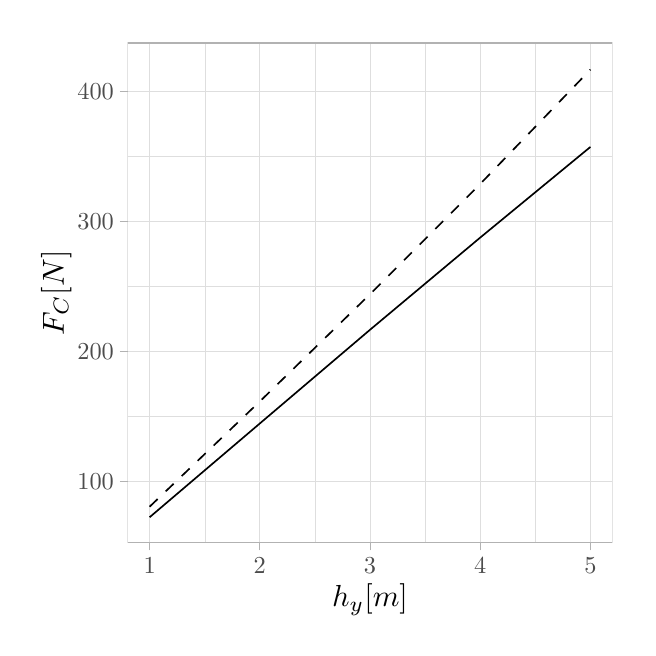
\begin{tikzpicture}[x=1pt,y=1pt]
\definecolor{fillColor}{RGB}{255,255,255}
\path[use as bounding box,fill=fillColor,fill opacity=0.00] (0,0) rectangle (216.81,216.81);
\begin{scope}
\path[clip] (  0.00,  0.00) rectangle (216.81,216.81);
\definecolor{drawColor}{RGB}{255,255,255}
\definecolor{fillColor}{RGB}{255,255,255}

\path[draw=drawColor,line width= 0.6pt,line join=round,line cap=round,fill=fillColor] (  0.00,  0.00) rectangle (216.81,216.81);
\end{scope}
\begin{scope}
\path[clip] ( 36.11, 30.69) rectangle (211.31,211.31);
\definecolor{fillColor}{RGB}{255,255,255}

\path[fill=fillColor] ( 36.11, 30.69) rectangle (211.31,211.31);
\definecolor{drawColor}{gray}{0.87}

\path[draw=drawColor,line width= 0.1pt,line join=round] ( 36.11, 76.43) --
	(211.31, 76.43);

\path[draw=drawColor,line width= 0.1pt,line join=round] ( 36.11,123.34) --
	(211.31,123.34);

\path[draw=drawColor,line width= 0.1pt,line join=round] ( 36.11,170.26) --
	(211.31,170.26);

\path[draw=drawColor,line width= 0.1pt,line join=round] ( 63.98, 30.69) --
	( 63.98,211.31);

\path[draw=drawColor,line width= 0.1pt,line join=round] (103.80, 30.69) --
	(103.80,211.31);

\path[draw=drawColor,line width= 0.1pt,line join=round] (143.62, 30.69) --
	(143.62,211.31);

\path[draw=drawColor,line width= 0.1pt,line join=round] (183.44, 30.69) --
	(183.44,211.31);

\path[draw=drawColor,line width= 0.3pt,line join=round] ( 36.11, 52.97) --
	(211.31, 52.97);

\path[draw=drawColor,line width= 0.3pt,line join=round] ( 36.11, 99.89) --
	(211.31, 99.89);

\path[draw=drawColor,line width= 0.3pt,line join=round] ( 36.11,146.80) --
	(211.31,146.80);

\path[draw=drawColor,line width= 0.3pt,line join=round] ( 36.11,193.72) --
	(211.31,193.72);

\path[draw=drawColor,line width= 0.3pt,line join=round] ( 44.07, 30.69) --
	( 44.07,211.31);

\path[draw=drawColor,line width= 0.3pt,line join=round] ( 83.89, 30.69) --
	( 83.89,211.31);

\path[draw=drawColor,line width= 0.3pt,line join=round] (123.71, 30.69) --
	(123.71,211.31);

\path[draw=drawColor,line width= 0.3pt,line join=round] (163.53, 30.69) --
	(163.53,211.31);

\path[draw=drawColor,line width= 0.3pt,line join=round] (203.35, 30.69) --
	(203.35,211.31);
\definecolor{drawColor}{RGB}{0,0,0}

\path[draw=drawColor,line width= 0.6pt,line join=round] ( 44.07, 39.91) --
	( 83.89, 73.79) --
	(123.71,107.65) --
	(163.53,140.96) --
	(203.35,173.72);

\path[draw=drawColor,line width= 0.6pt,dash pattern=on 4pt off 4pt ,line join=round] ( 44.07, 43.72) --
	( 83.89, 81.75) --
	(123.71,120.50) --
	(163.53,160.34) --
	(203.35,201.65);
\definecolor{drawColor}{gray}{0.70}

\path[draw=drawColor,line width= 0.6pt,line join=round,line cap=round] ( 36.11, 30.69) rectangle (211.31,211.31);
\end{scope}
\begin{scope}
\path[clip] (  0.00,  0.00) rectangle (216.81,216.81);
\definecolor{drawColor}{gray}{0.30}

\node[text=drawColor,anchor=base east,inner sep=0pt, outer sep=0pt, scale=  0.88] at ( 31.16, 49.94) {100};

\node[text=drawColor,anchor=base east,inner sep=0pt, outer sep=0pt, scale=  0.88] at ( 31.16, 96.86) {200};

\node[text=drawColor,anchor=base east,inner sep=0pt, outer sep=0pt, scale=  0.88] at ( 31.16,143.77) {300};

\node[text=drawColor,anchor=base east,inner sep=0pt, outer sep=0pt, scale=  0.88] at ( 31.16,190.69) {400};
\end{scope}
\begin{scope}
\path[clip] (  0.00,  0.00) rectangle (216.81,216.81);
\definecolor{drawColor}{gray}{0.70}

\path[draw=drawColor,line width= 0.3pt,line join=round] ( 33.36, 52.97) --
	( 36.11, 52.97);

\path[draw=drawColor,line width= 0.3pt,line join=round] ( 33.36, 99.89) --
	( 36.11, 99.89);

\path[draw=drawColor,line width= 0.3pt,line join=round] ( 33.36,146.80) --
	( 36.11,146.80);

\path[draw=drawColor,line width= 0.3pt,line join=round] ( 33.36,193.72) --
	( 36.11,193.72);
\end{scope}
\begin{scope}
\path[clip] (  0.00,  0.00) rectangle (216.81,216.81);
\definecolor{drawColor}{gray}{0.70}

\path[draw=drawColor,line width= 0.3pt,line join=round] ( 44.07, 27.94) --
	( 44.07, 30.69);

\path[draw=drawColor,line width= 0.3pt,line join=round] ( 83.89, 27.94) --
	( 83.89, 30.69);

\path[draw=drawColor,line width= 0.3pt,line join=round] (123.71, 27.94) --
	(123.71, 30.69);

\path[draw=drawColor,line width= 0.3pt,line join=round] (163.53, 27.94) --
	(163.53, 30.69);

\path[draw=drawColor,line width= 0.3pt,line join=round] (203.35, 27.94) --
	(203.35, 30.69);
\end{scope}
\begin{scope}
\path[clip] (  0.00,  0.00) rectangle (216.81,216.81);
\definecolor{drawColor}{gray}{0.30}

\node[text=drawColor,anchor=base,inner sep=0pt, outer sep=0pt, scale=  0.88] at ( 44.07, 19.68) {1};

\node[text=drawColor,anchor=base,inner sep=0pt, outer sep=0pt, scale=  0.88] at ( 83.89, 19.68) {2};

\node[text=drawColor,anchor=base,inner sep=0pt, outer sep=0pt, scale=  0.88] at (123.71, 19.68) {3};

\node[text=drawColor,anchor=base,inner sep=0pt, outer sep=0pt, scale=  0.88] at (163.53, 19.68) {4};

\node[text=drawColor,anchor=base,inner sep=0pt, outer sep=0pt, scale=  0.88] at (203.35, 19.68) {5};
\end{scope}
\begin{scope}
\path[clip] (  0.00,  0.00) rectangle (216.81,216.81);
\definecolor{drawColor}{RGB}{0,0,0}

\node[text=drawColor,anchor=base,inner sep=0pt, outer sep=0pt, scale=  1.10] at (123.71,  7.64) {$h_y [m]$};
\end{scope}
\begin{scope}
\path[clip] (  0.00,  0.00) rectangle (216.81,216.81);
\definecolor{drawColor}{RGB}{0,0,0}

\node[text=drawColor,rotate= 90.00,anchor=base,inner sep=0pt, outer sep=0pt, scale=  1.10] at ( 13.08,121.00) {$F_C [N]$};
\end{scope}
\end{tikzpicture}
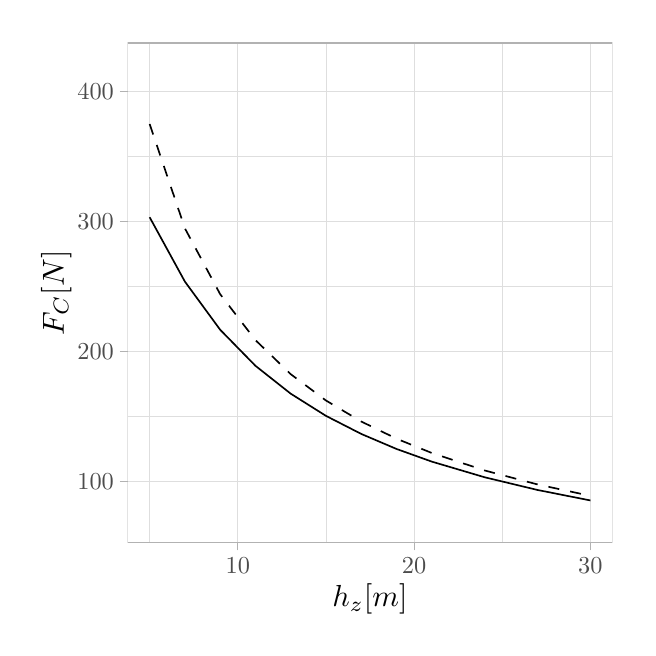
\begin{tikzpicture}[x=1pt,y=1pt]
\definecolor{fillColor}{RGB}{255,255,255}
\path[use as bounding box,fill=fillColor,fill opacity=0.00] (0,0) rectangle (216.81,216.81);
\begin{scope}
\path[clip] (  0.00,  0.00) rectangle (216.81,216.81);
\definecolor{drawColor}{RGB}{255,255,255}
\definecolor{fillColor}{RGB}{255,255,255}

\path[draw=drawColor,line width= 0.6pt,line join=round,line cap=round,fill=fillColor] (  0.00,  0.00) rectangle (216.81,216.81);
\end{scope}
\begin{scope}
\path[clip] ( 36.11, 30.69) rectangle (211.31,211.31);
\definecolor{fillColor}{RGB}{255,255,255}

\path[fill=fillColor] ( 36.11, 30.69) rectangle (211.31,211.31);
\definecolor{drawColor}{gray}{0.87}

\path[draw=drawColor,line width= 0.1pt,line join=round] ( 36.11, 76.43) --
	(211.31, 76.43);

\path[draw=drawColor,line width= 0.1pt,line join=round] ( 36.11,123.34) --
	(211.31,123.34);

\path[draw=drawColor,line width= 0.1pt,line join=round] ( 36.11,170.26) --
	(211.31,170.26);

\path[draw=drawColor,line width= 0.1pt,line join=round] ( 44.07, 30.69) --
	( 44.07,211.31);

\path[draw=drawColor,line width= 0.1pt,line join=round] (107.78, 30.69) --
	(107.78,211.31);

\path[draw=drawColor,line width= 0.1pt,line join=round] (171.49, 30.69) --
	(171.49,211.31);

\path[draw=drawColor,line width= 0.3pt,line join=round] ( 36.11, 52.97) --
	(211.31, 52.97);

\path[draw=drawColor,line width= 0.3pt,line join=round] ( 36.11, 99.89) --
	(211.31, 99.89);

\path[draw=drawColor,line width= 0.3pt,line join=round] ( 36.11,146.80) --
	(211.31,146.80);

\path[draw=drawColor,line width= 0.3pt,line join=round] ( 36.11,193.72) --
	(211.31,193.72);

\path[draw=drawColor,line width= 0.3pt,line join=round] ( 75.93, 30.69) --
	( 75.93,211.31);

\path[draw=drawColor,line width= 0.3pt,line join=round] (139.64, 30.69) --
	(139.64,211.31);

\path[draw=drawColor,line width= 0.3pt,line join=round] (203.35, 30.69) --
	(203.35,211.31);
\definecolor{drawColor}{RGB}{0,0,0}

\path[draw=drawColor,line width= 0.6pt,line join=round] ( 44.07,148.32) --
	( 56.82,125.04) --
	( 69.56,107.65) --
	( 82.30, 94.63) --
	( 95.04, 84.56) --
	(107.78, 76.54) --
	(120.53, 70.01) --
	(133.27, 64.58) --
	(146.01, 60.01) --
	(165.12, 54.35) --
	(184.23, 49.76) --
	(203.35, 45.97);

\path[draw=drawColor,line width= 0.6pt,dash pattern=on 4pt off 4pt ,line join=round] ( 44.07,181.99) --
	( 56.82,144.28) --
	( 69.56,120.50) --
	( 82.30,103.91) --
	( 95.04, 91.61) --
	(107.78, 82.09) --
	(120.53, 74.50) --
	(133.27, 68.29) --
	(146.01, 63.13) --
	(165.12, 56.81) --
	(184.23, 51.76) --
	(203.35, 47.63);
\definecolor{drawColor}{gray}{0.70}

\path[draw=drawColor,line width= 0.6pt,line join=round,line cap=round] ( 36.11, 30.69) rectangle (211.31,211.31);
\end{scope}
\begin{scope}
\path[clip] (  0.00,  0.00) rectangle (216.81,216.81);
\definecolor{drawColor}{gray}{0.30}

\node[text=drawColor,anchor=base east,inner sep=0pt, outer sep=0pt, scale=  0.88] at ( 31.16, 49.94) {100};

\node[text=drawColor,anchor=base east,inner sep=0pt, outer sep=0pt, scale=  0.88] at ( 31.16, 96.86) {200};

\node[text=drawColor,anchor=base east,inner sep=0pt, outer sep=0pt, scale=  0.88] at ( 31.16,143.77) {300};

\node[text=drawColor,anchor=base east,inner sep=0pt, outer sep=0pt, scale=  0.88] at ( 31.16,190.69) {400};
\end{scope}
\begin{scope}
\path[clip] (  0.00,  0.00) rectangle (216.81,216.81);
\definecolor{drawColor}{gray}{0.70}

\path[draw=drawColor,line width= 0.3pt,line join=round] ( 33.36, 52.97) --
	( 36.11, 52.97);

\path[draw=drawColor,line width= 0.3pt,line join=round] ( 33.36, 99.89) --
	( 36.11, 99.89);

\path[draw=drawColor,line width= 0.3pt,line join=round] ( 33.36,146.80) --
	( 36.11,146.80);

\path[draw=drawColor,line width= 0.3pt,line join=round] ( 33.36,193.72) --
	( 36.11,193.72);
\end{scope}
\begin{scope}
\path[clip] (  0.00,  0.00) rectangle (216.81,216.81);
\definecolor{drawColor}{gray}{0.70}

\path[draw=drawColor,line width= 0.3pt,line join=round] ( 75.93, 27.94) --
	( 75.93, 30.69);

\path[draw=drawColor,line width= 0.3pt,line join=round] (139.64, 27.94) --
	(139.64, 30.69);

\path[draw=drawColor,line width= 0.3pt,line join=round] (203.35, 27.94) --
	(203.35, 30.69);
\end{scope}
\begin{scope}
\path[clip] (  0.00,  0.00) rectangle (216.81,216.81);
\definecolor{drawColor}{gray}{0.30}

\node[text=drawColor,anchor=base,inner sep=0pt, outer sep=0pt, scale=  0.88] at ( 75.93, 19.68) {10};

\node[text=drawColor,anchor=base,inner sep=0pt, outer sep=0pt, scale=  0.88] at (139.64, 19.68) {20};

\node[text=drawColor,anchor=base,inner sep=0pt, outer sep=0pt, scale=  0.88] at (203.35, 19.68) {30};
\end{scope}
\begin{scope}
\path[clip] (  0.00,  0.00) rectangle (216.81,216.81);
\definecolor{drawColor}{RGB}{0,0,0}

\node[text=drawColor,anchor=base,inner sep=0pt, outer sep=0pt, scale=  1.10] at (123.71,  7.64) {$h_z [m]$};
\end{scope}
\begin{scope}
\path[clip] (  0.00,  0.00) rectangle (216.81,216.81);
\definecolor{drawColor}{RGB}{0,0,0}

\node[text=drawColor,rotate= 90.00,anchor=base,inner sep=0pt, outer sep=0pt, scale=  1.10] at ( 13.08,121.00) {$F_C [N]$};
\end{scope}
\end{tikzpicture}
